\subsection{Kiến trúc hệ thống}

\subsubsection{Quản lý các thông tin bí mật (Doppler)}

Quản lý các thông tin bí mật là một phần cực kỳ quan trọng. Đặc biệt khi hệ thống được thiết kế theo kiến trúc microservices.
Khi dự án có nhiều dịch vụ, việc sử dụng file .env độc lập cho từng dịch vụ sẽ gây khó khăn trong việc quản lý, cấu hình, đồng bộ và bảo mật.

\begin{figure}[H]
\centering
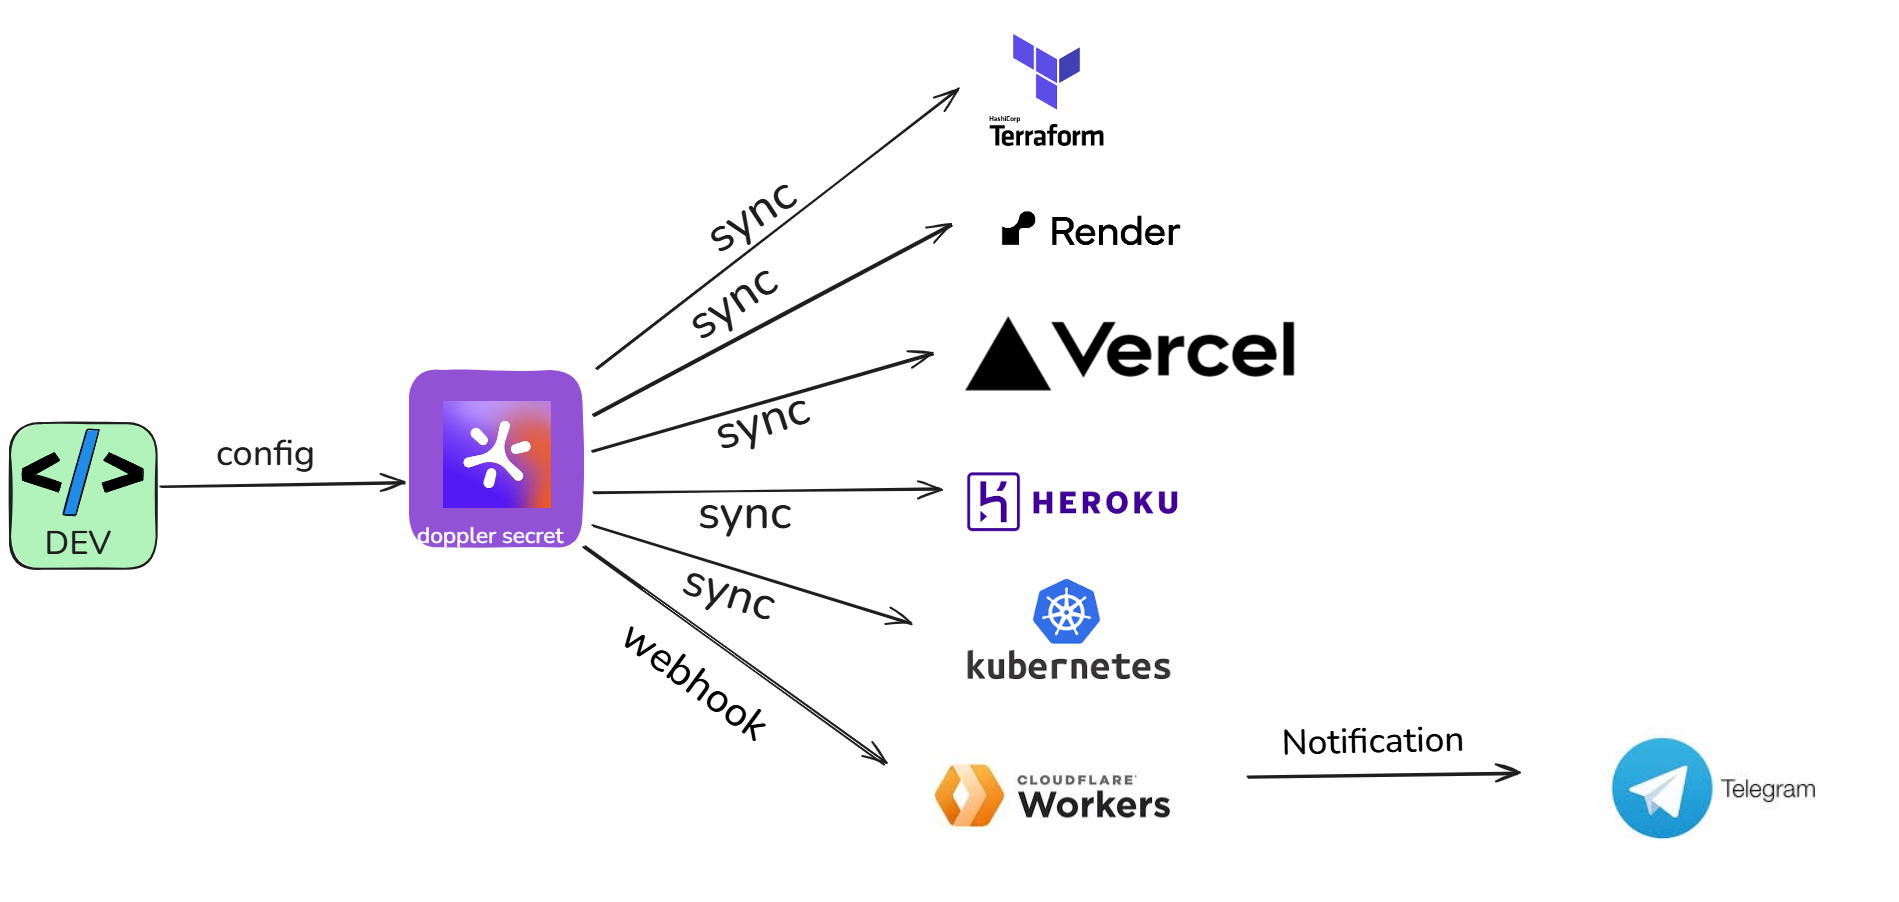
\includegraphics[width=0.95\textwidth]{pictures/secret-by-doppler.excalidraw.png}
\caption{Sơ đồ quản lý secret bằng Doppler}
\end{figure}

% \begin{block}{Ứng dụng trong đồ án}
Trong đồ án này, em sử dụng Doppler
% - một nền tảng
quản lý thông tin bí mật tập trung.
Việc áp dụng Doppler mang lại một không gian lưu trữ an toàn,
thống nhất (Single Source of Truth) cho toàn bộ hệ thống.
Các
bí mật
được
chia nhỏ theo từng nhu cầu sử dụng trong Doppler.

\begin{figure}[H]
\centering
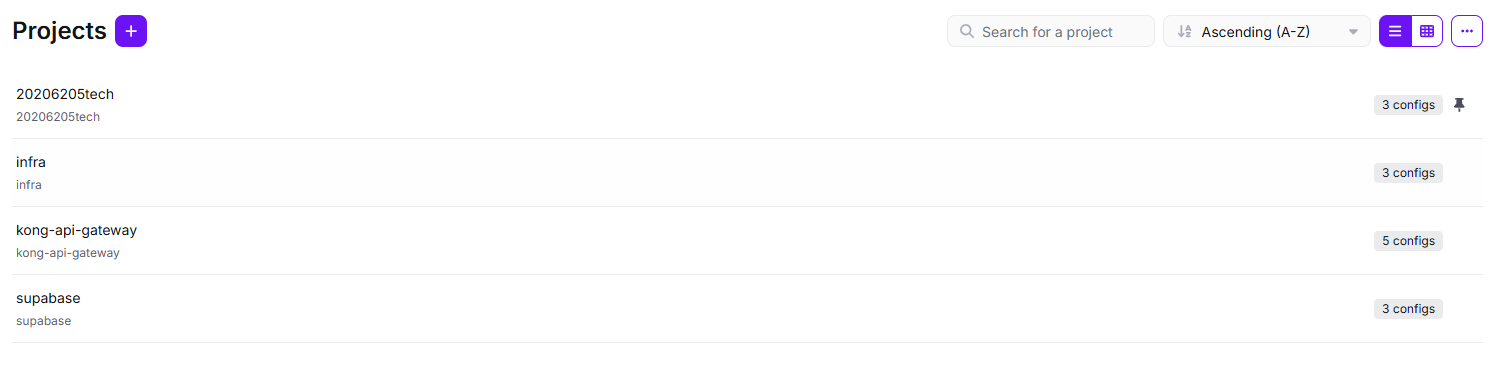
\includegraphics[width=0.95\textwidth]{pictures/doppler-projects.png}
\caption{Cấu hình chia nhỏ bí mật theo từng nhu cầu sử dụng trong Doppler}
\end{figure}

Trong hệ thống Doppler, bản miễn phí có hỗ trợ nhánh dev personal riêng cho từng lập trình viên, từng cá nhân có thể ghi đè hoặc thêm các biến mà không làm ảnh hưởng đến cấu hình chung. Trong bản trả phí, Doppler hỗ trợ tính năng xoay vòng tự động các biến bí mật.

\begin{figure}[H]
\centering
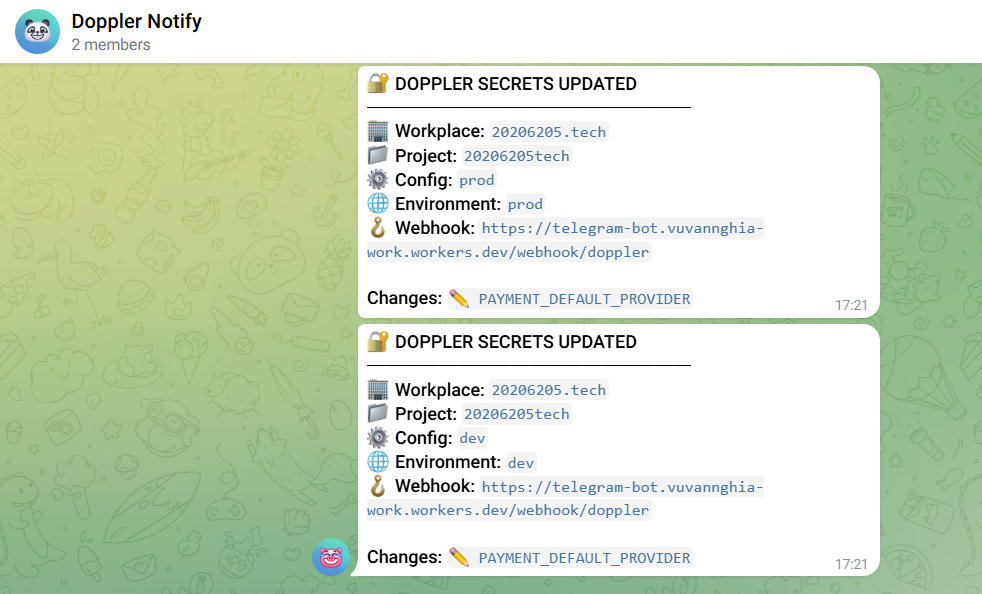
\includegraphics[width=0.6\textwidth]{pictures/doppler-telegram2.png}
\caption{Kết quả thông báo telegram khi Doppler có sự thay đổi}
\end{figure}
